%----------------------------------------------------------------------------------------
%	PACKAGES AND DOCUMENT CONFIGURATIONS
%----------------------------------------------------------------------------------------

\documentclass{article}
\usepackage{indentfirst}

\usepackage{booktabs} %需要加载宏包{booktabs}
\usepackage{fontawesome}
\usepackage{graphicx} % Required for the inclusion of images
\usepackage{subfigure} % Required for the inclusion of images
\usepackage{natbib} % Required to change bibliography style to APA
\usepackage{amsmath} % Required for some math elements 
\usepackage{marvosym}
\usepackage{color,amsmath,amssymb,graphicx,fancyhdr,amsfonts,amsthm,algorithmic,verbatim,bbold}
\usepackage{tikz}
\usetikzlibrary{graphs, positioning, quotes, shapes.geometric}
  \usepackage{listings}
  \newcommand{\Rmnum}[1]{\uppercase\expandafter{\romannumeral #1}}  %定义命令输入大写罗马数字
  \newcommand{\rmnum}[1]{\romannumeral #1}  %定义命令输入小写罗马数字
  
 \usepackage{hyperref}
 \hypersetup{hidelinks,
 	colorlinks=true,
 	allcolors=black,
 	pdfstartview=Fit,
 	breaklinks=true}
  
  
  \lstset{
language=bash,
basicstyle=\ttfamily,
numbers=left,
numbersep=5pt,
xleftmargin=20pt,
frame=tb,
framexleftmargin=20pt,
keywordstyle=\color{blue}\bfseries,
%commentstyle=\color{dkgreen},
commentstyle=\color{gray!80}\textit,
stringstyle=\color{red!100!green!50!blue!100},
breaklines=true,
%breakatwhitespace=true,
escapeinside=``,%逃逸字符(1左面的键),用于显示中文例如在代码中`中文...`
tabsize=4,
extendedchars=false,
aboveskip=3mm,
belowskip=3mm,
showstringspaces=false,
columns=flexible,
}


%\usepackage{times} % Uncomment to use the Times New Roman font

%----------------------------------------------------------------------------------------
%	DOCUMENT INFORMATION
%----------------------------------------------------------------------------------------

\title{\textbf{Project 2: OFDM MATLAB Simulation}} % Title

\author{Zhuohao Lee~\textsuperscript{\Letter }\thanks{edith$\_$lzh@sjtu.edu.cn | 519021911248 | \faGithub{}{\underline{\href{https://github.com/edithlzh/VLSI-course-note}{~Project Repo}}}}} % Author name and email

\date{\today} % Date for the report

\begin{document}

\maketitle % Insert the title, author and date

\tableofcontents

\newpage

\section{Introduction}
OFDM is a special multi-carrier transmission scheme, which can be regarded as a modulation technology or as a multiplexing technology.

Simply put: OFDM is a multi-carrier transmission method, which divides the frequency band into multiple sub-channels to transmit data in parallel, divides the high-speed data stream into multiple parallel low-speed data streams, and then modulates to the sub-carriers of each channel for transmission. Because it converts non-flat fading wireless channels into multiple orthogonal flat fading sub-channels, it can eliminate the interference between channel waveforms and achieve the purpose of combating multipath fading.

Orthogonal Frequency Division Multiplexing (OFDM) is an improvement on multi-carrier modulation (MCM) in. Its characteristic is that each subcarrier is orthogonal to each other, so the spectrum after spread spectrum modulation can overlap each other, which not only reduces the mutual interference between subcarriers, but also greatly improves the spectrum utilization rate.

A big reason for choosing OFDM is that the system can resist frequency selective fading and narrowband interference well. In a single carrier system, one fading or interference will cause the entire link to fail, but in a multi-carrier system, only a small number of subchannels will be affected by deep fading at a certain time.

\textbf{This lab is finished individually by \underline{Zhuohao}}


\section{Lab}
\subsection{Digital baseband modulation and demodulation \& Simulation of OFDM Communication System}
\subsubsection{Analysis}


Attached file \lstinline|./ofdm.m| is the source code I'll refer to in this lab.

In this lab, we select channel as \textbf{AWGN}, and did modulation with \textbf{BPSK, QPSK, 16-QAM, 64-QAM}. Through Monte Carlo simulation, the performance of various modulation methods is verified, and MATLAB tools BER comparison is carried out bertool the obtained theoretical values to verify the correctness of the simulation.I n this part, we're gonna write and test the performance of the system under 16/64 QAM modulation and compare it with the theoretical curve. And we're gonna analyze the performance, advantages and disadvantages of various modulation and demodulation methods.

We'll use \textbf{IEEE 802.11a} protocol. As for its configuration, 48 subcarriers are used to transmit data, 4 subcarriers are used for pilot symbols (pilot symbols are zero in this experiment),12 subcarriers are empty (input zero is enough),OFDM configuration is completed in the OFDM mapping module in fig. 1, which is described in detail in the appendix. A total of 64 subcarriers, 64 points of IFFT/FFT.

\begin{figure}[!h]
	\centering
	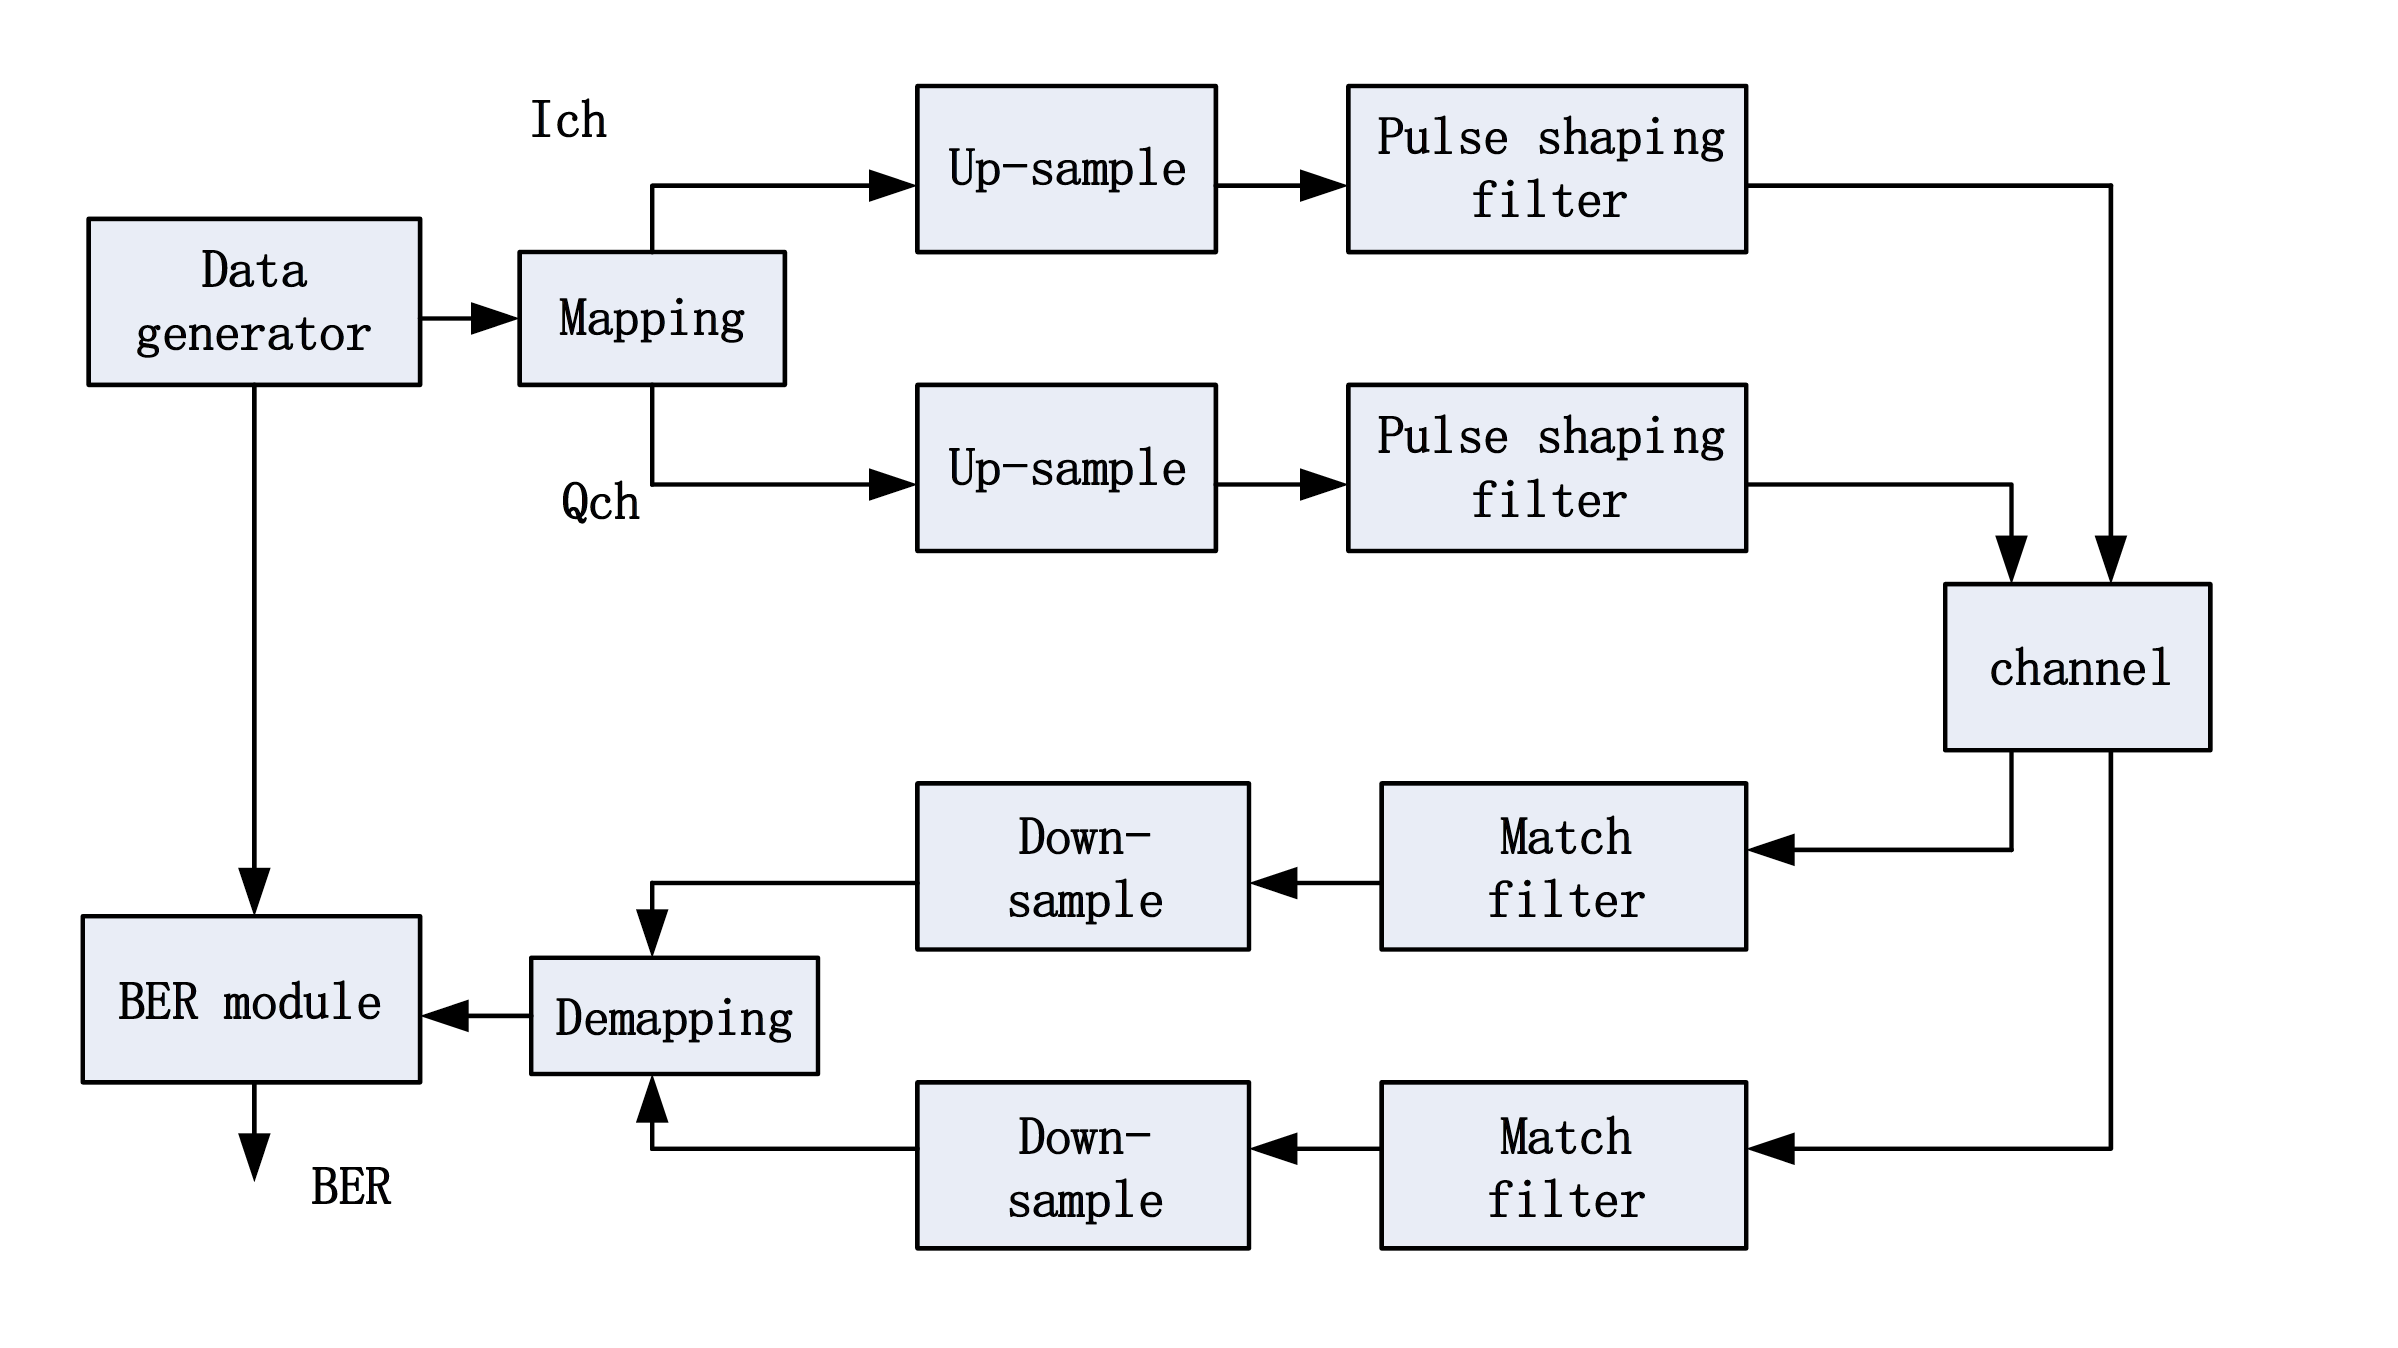
\includegraphics[width=0.7\linewidth]{1}
	\caption{Modulation and demodulation -  System block diagram}
	\label{fig:1}
\end{figure}
\begin{figure}[!h]
	\centering
	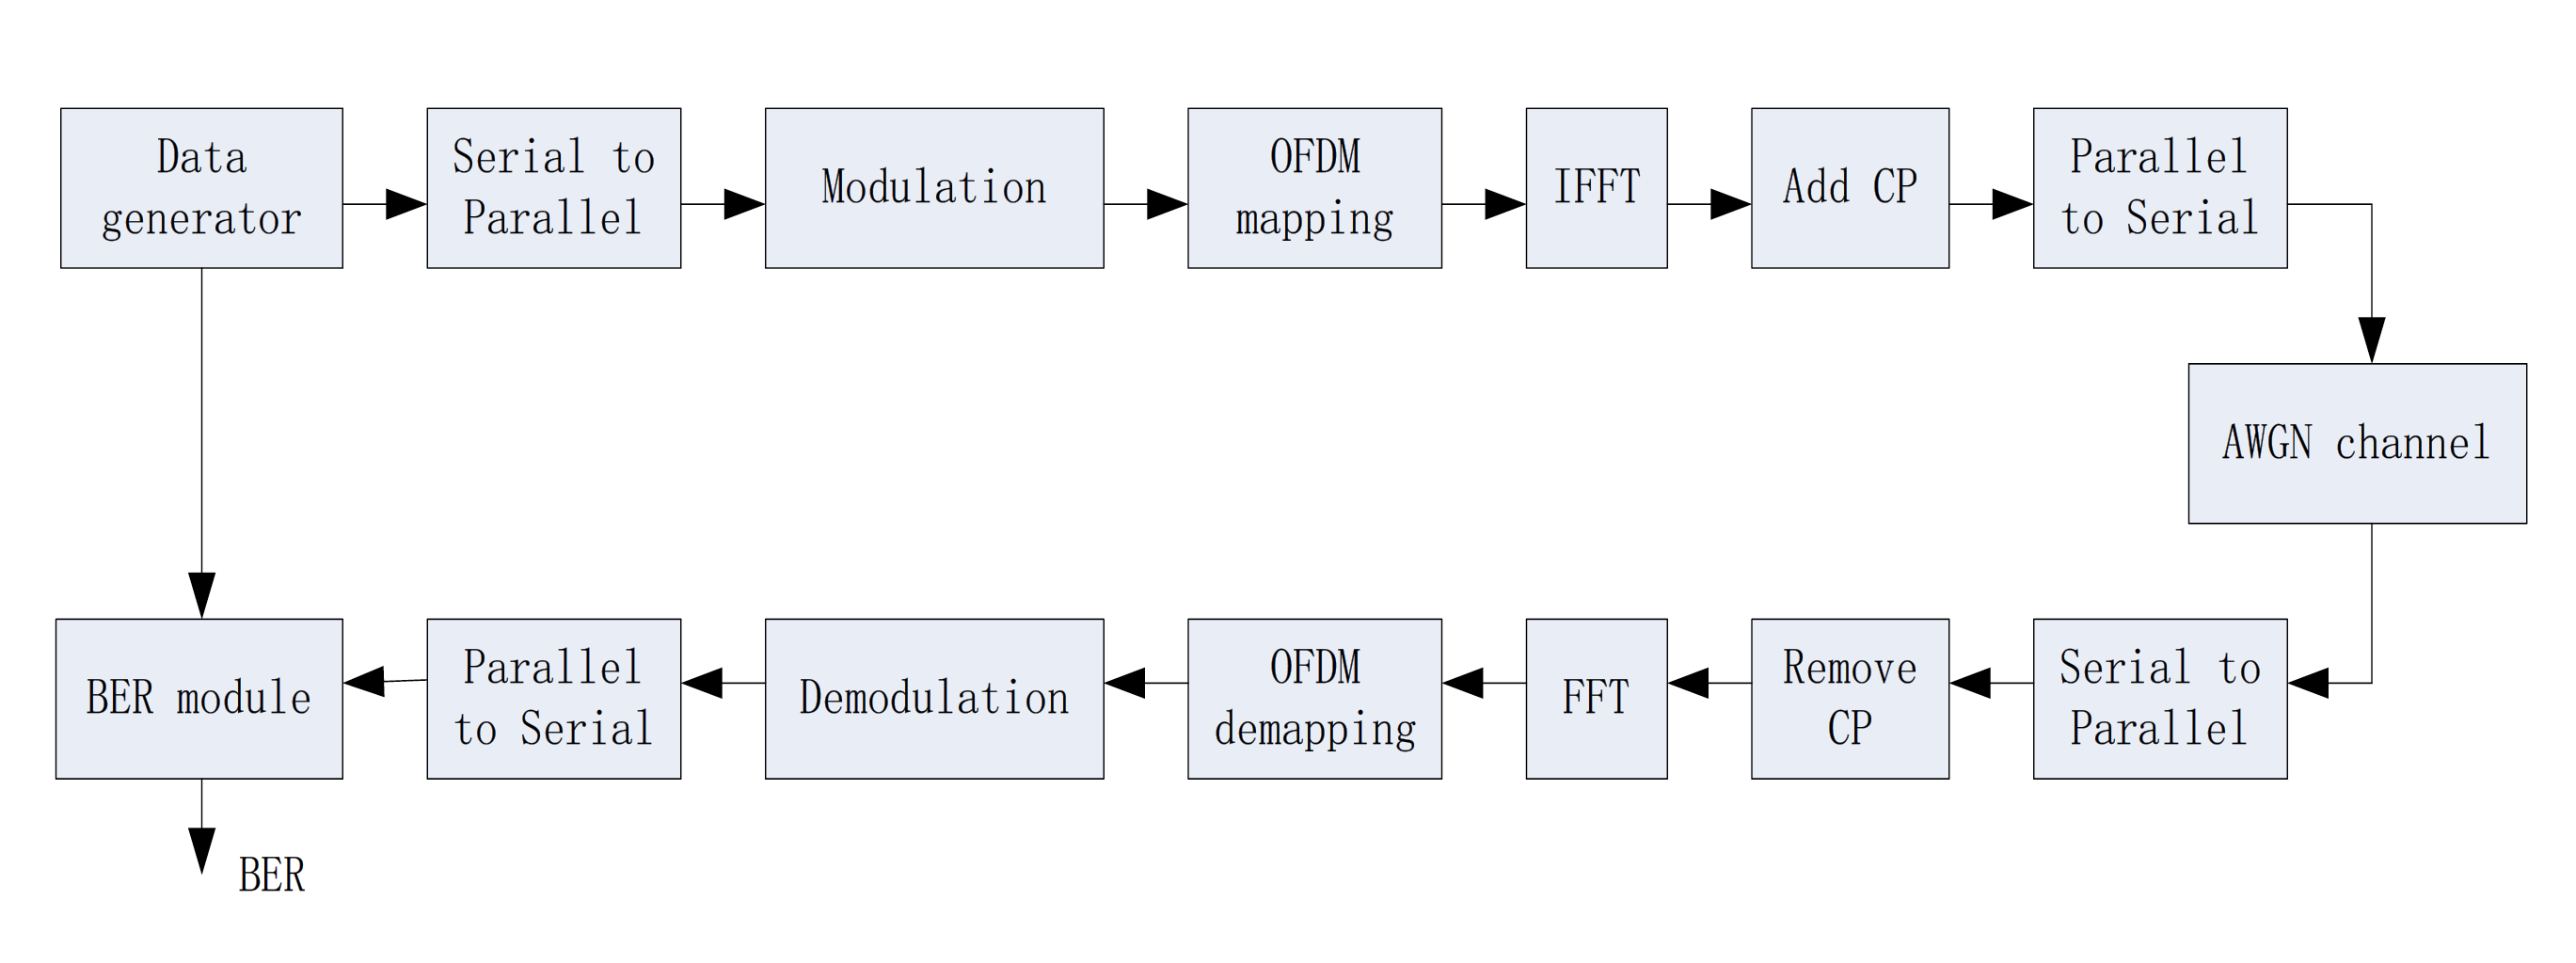
\includegraphics[width=0.7\linewidth]{2}
	\caption{OFDM - System block diagram}
	\label{fig:2}
\end{figure}

\subsubsection{Code}

\textbf{\textcolor{blue}{Modulation}}

\lstinline|ofdm.m| is the main function used in this lab and we're gonna modify \lstinline|ofdmmod.m| and \lstinline|ofdmdemod.m| to implement specifc modulation and demodulation.

Reffered to lecture notes and constellation figure of 16-QAM and 64-QAM. The \lstinline|ofdmmod.m| shows like below:

\begin{lstlisting}
switch (OFDM.mod_lev)
	case 1 % BPSK
		OFDM.Constellations = [-1, 1];
	case 2 % 4-QAM / QPSK
		OFDM.Constellations = [-1- 1i, -1+1i, ...
									+1-1i, +1+1i];
	case 4 % 16-QAM
		OFDM.Constellations = [-3-3i, -3-1i, -3+1i, -3+3i, ...
									-1+3i, -1+1i, -1-1i, -1-3i, ...
									1-3i , 1-1i , 1+1i , 1+3i , ...
									3+3i , 3+1i , 3-1i , 3-3i]; 
									% you should fix it;
	case 6 % 64-QAM
		OFDM.Constellations = [-7-7i, -7-5i, -7-3i, -7-1i, ...
									-7+1i, -7+3i, -7+5i, -7+7i, ...
									-5+7i, -5+5i, -5+3i, -5+1i, ...
									-5-1i, -5-3i, -5-5i, -5-7i, ...
									-3-7i, -3-5i, -3-3i, -3-1i, ...
									-3+1i, -3+3i, -3+5i, -3+7i, ...
									-1-7i, -1-5i, -1-3i, -1-1i, ...
									-1+1i, -1+3i, -1+5i, -1+7i, ...
									1+7i, 1+5i, 1+3i, 1+1i,  ...
									1-1i, 1-3i, 1-5i, 1-7i,  ...
									3-7i, 3-5i, 3-3i, 3-1i,  ...
									3+1i, 3+3i, 3+5i, 3+7i,  ...
									5+7i, 5+5i, 5+3i, 5+1i,  ...
									5-1i, 5-3i, 5-5i, 5-7i,  ...
									7-7i, 7-5i, 7-3i, 7-1i,  ...
									7+1i, 7+3i, 7+5i, 7+7i,  ]; 
									% you should fix it;
\end{lstlisting}

\textbf{\textcolor{blue}{Demodulation}}

The basic idea to do demodulation is  \textbf{iteration} and \textbf{condition}. Here I only take \lstinline|qam16demod| as an example. 

\begin{lstlisting}
demodata=zeros(para,ml*nd); % output data
bitcount=ml/2; % which is 3 in 16-QAM
count=1; % counter 

for ii=1:nd %from 1 to 6
	for jj=1:para % from 1 to 48
%*********************************************************************
		if(idata(jj,ii)<-6)
			demodata(jj,count:count+bitcount-1)=[0,0,0];
		elseif((idata(jj,ii)>=-6)&&(idata(jj,ii)<-4))
			demodata(jj,count:count+bitcount-1)=[0,0,1];
		elseif((idata(jj,ii)>=-4)&&(idata(jj,ii)<-2))
			demodata(jj,count:count+bitcount-1)=[0,1,1];
		elseif((idata(jj,ii)>=-2)&&(idata(jj,ii)<0))
			demodata(jj,count:count+bitcount-1)=[0,1,0];
		elseif((idata(jj,ii)>=0)&&(idata(jj,ii)<2))
			demodata(jj,count:count+bitcount-1)=[1,1,0];
		elseif((idata(jj,ii)>=2)&&(idata(jj,ii)<4))
			demodata(jj,count:count+bitcount-1)=[1,1,1];
		elseif((idata(jj,ii)>=4)&&(idata(jj,ii)<6))
			demodata(jj,count:count+bitcount-1)=[1,0,1];
		else
			demodata(jj,count:count+bitcount-1)=[1,0,0];
		end
		
		if(qdata(jj,ii)<-6)
			demodata(jj,count+bitcount:count+ml-1)=[0,0,0];
		elseif((qdata(jj,ii)>=-6)&&(qdata(jj,ii)<-4))
			demodata(jj,count+bitcount:count+ml-1)=[0,0,1];
		elseif((qdata(jj,ii)>=-4)&&(qdata(jj,ii)<-2))
			demodata(jj,count+bitcount:count+ml-1)=[0,1,1];
		elseif((qdata(jj,ii)>=-2)&&(qdata(jj,ii)<0))
			demodata(jj,count+bitcount:count+ml-1)=[0,1,0];
		elseif((qdata(jj,ii)>=0)&&(qdata(jj,ii)<2))
			demodata(jj,count+bitcount:count+ml-1)=[1,1,0];
		elseif((qdata(jj,ii)>=2)&&(qdata(jj,ii)<4))
			demodata(jj,count+bitcount:count+ml-1)=[1,1,1];
		elseif((qdata(jj,ii)>=4)&&(qdata(jj,ii)<6))
			demodata(jj,count+bitcount:count+ml-1)=[1,0,1];
		else
			demodata(jj,count+bitcount:count+ml-1)=[1,0,0];
		end
	end
	count=count+ml;
end
\end{lstlisting}

\begin{center}
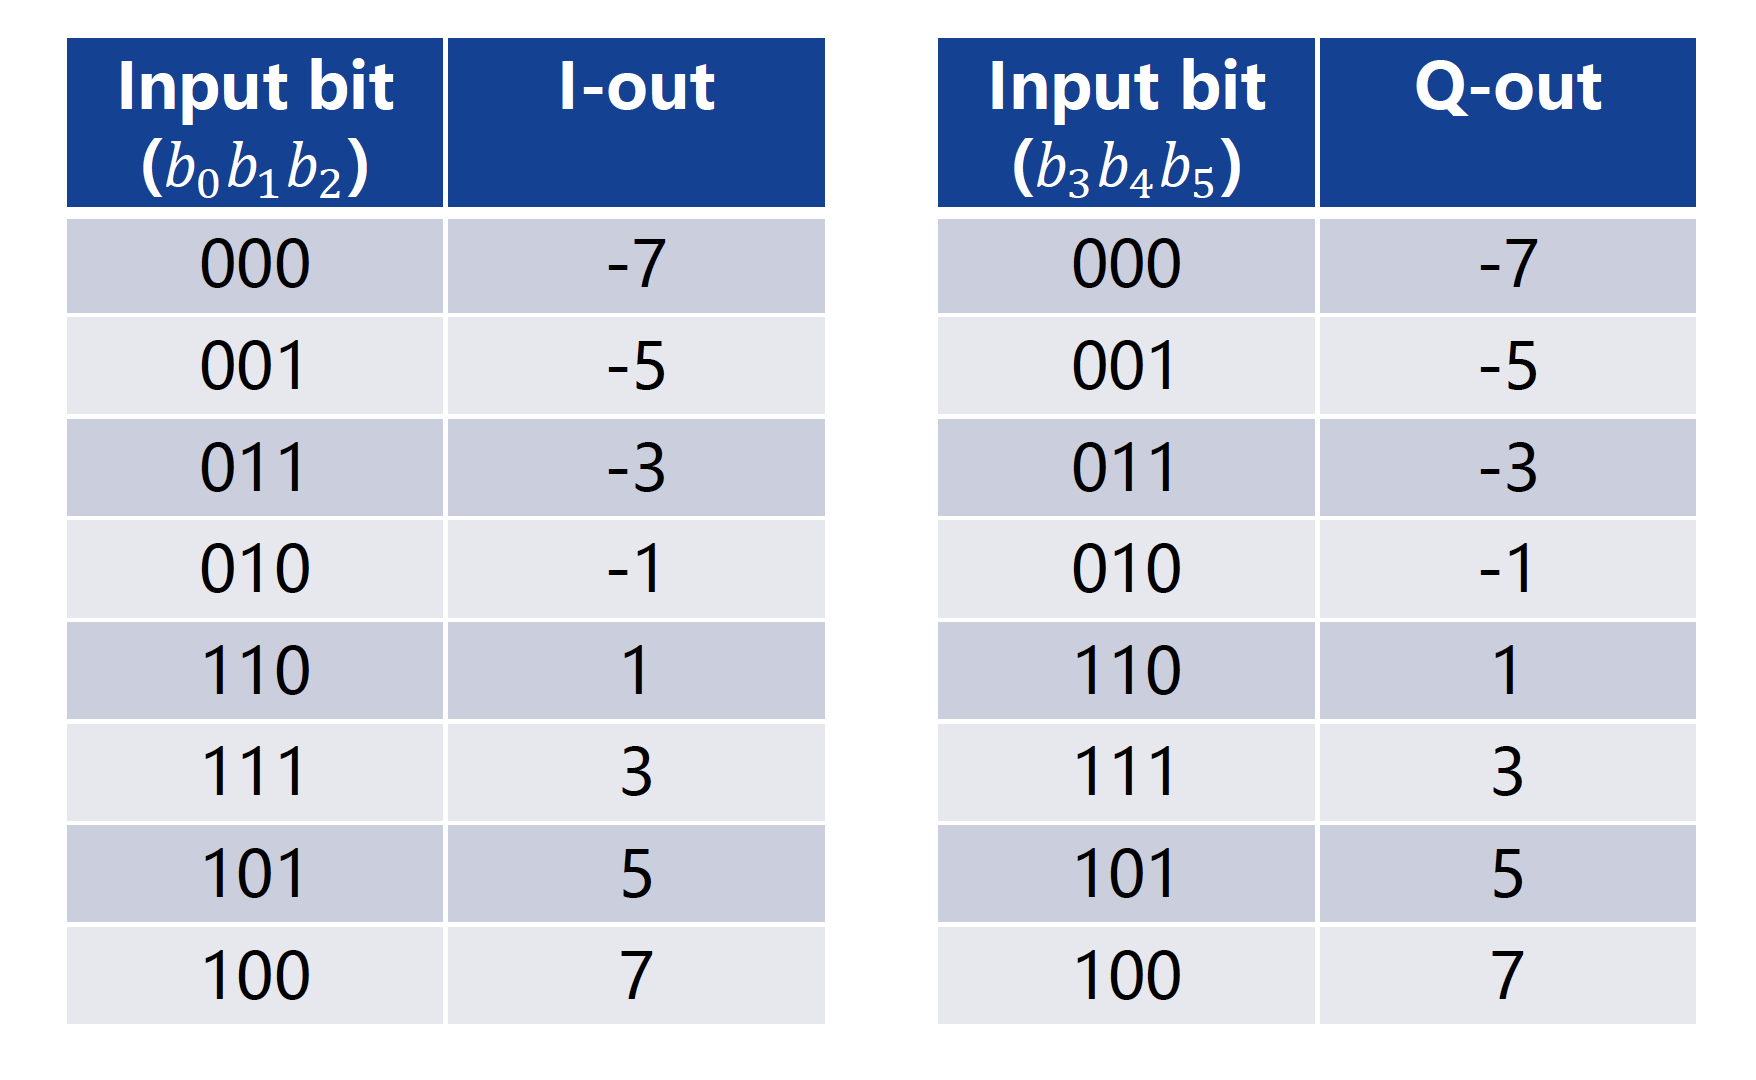
\includegraphics[width=10cm]{000}
\end{center}

Following the encode table mentioned above. Just do the corresponding condition then we can get the correct simulation result.

\textcolor{blue}{Vetorization to Speed Up}

We can also use vectorization technique to speed it up. MATLAB is very good at matrix or vectors operations like Pytorch or Tensorflow. By vectorizing the variables you can have bonus on efficiency.

\subsubsection{Result}

\textcolor{blue}{Theorical curve} is generated by \lstinline|bertools| just following lectures assigned. ( select modulation way $ \rightarrow $ plot $ \rightarrow $ export data ).

And the following results are listed:

\begin{itemize}
	\item \textbf{BPSK}
	
	\begin{figure}[!h]
		\centering
		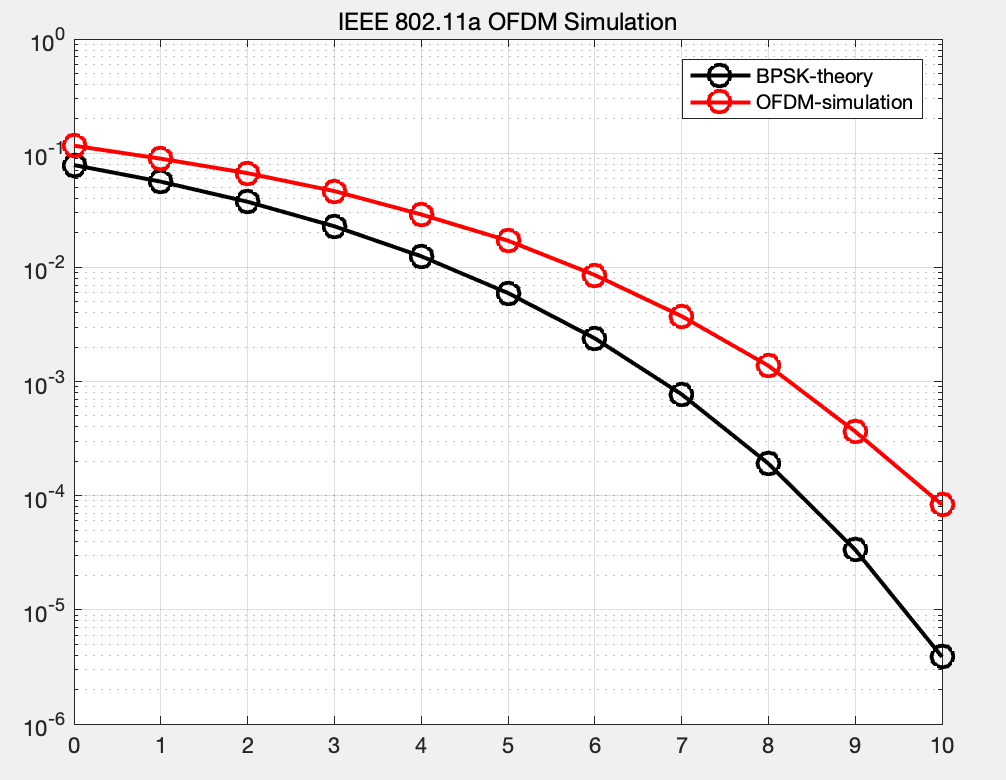
\includegraphics[width=0.7\linewidth]{B}
		\caption{BPSK}
		\label{fig:b}
	\end{figure}
	
	The BPSK result is shown as Fig.3. 
	\item  
	\textbf{QPSK}
	
	\begin{figure}[!h]
		\centering
		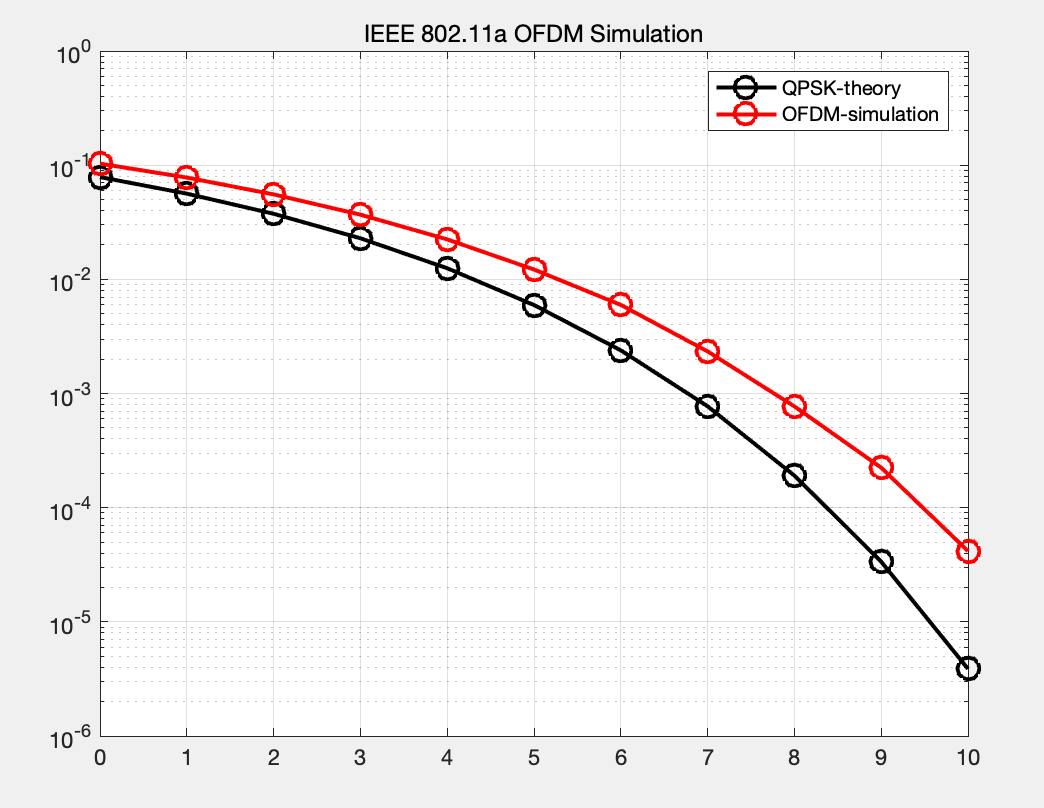
\includegraphics[width=0.7\linewidth]{Q}
		\caption{QPSK}
		\label{fig:q}
	\end{figure}
	The QPSK result is shown as Fig.4. 
	
	\item 
	\textbf{16-QAM}
	
	\begin{figure}[!h]
		\centering
		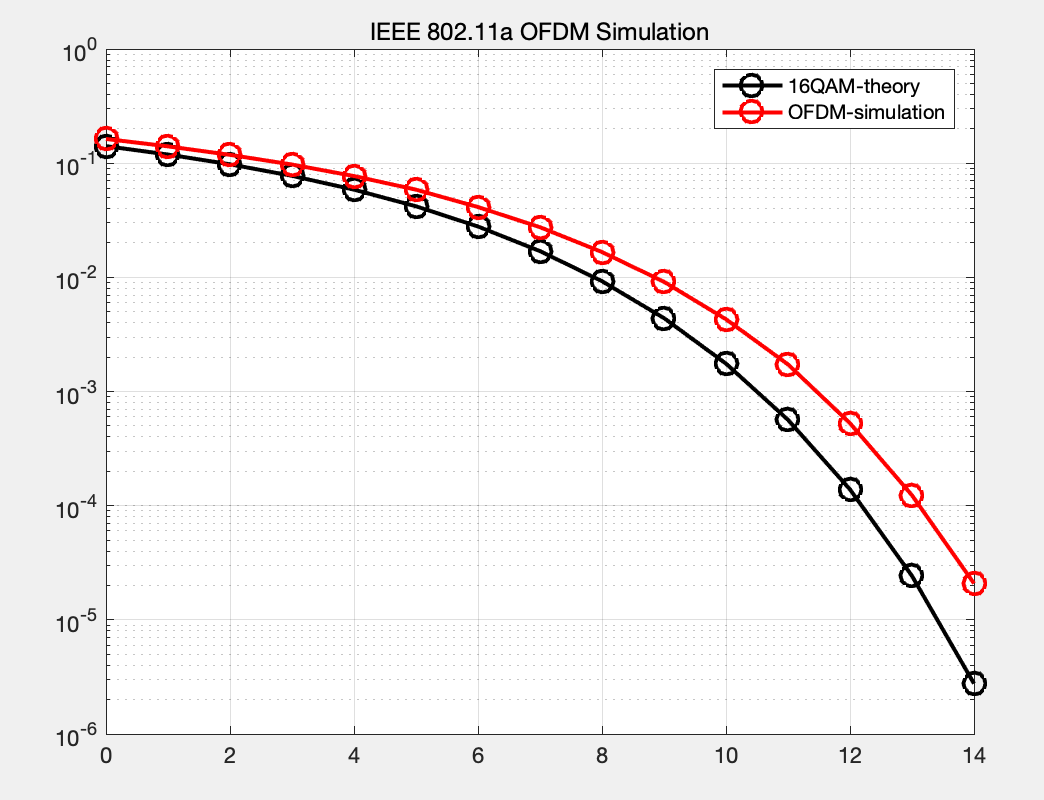
\includegraphics[width=0.7\linewidth]{16}
		\caption{16-QAM}
		\label{fig:16}
	\end{figure}
	
	The 16-QAM result is shown as Fig.5. 
	\item  
	\textbf{64-QAM}
	\begin{figure}[!h]
		\centering
		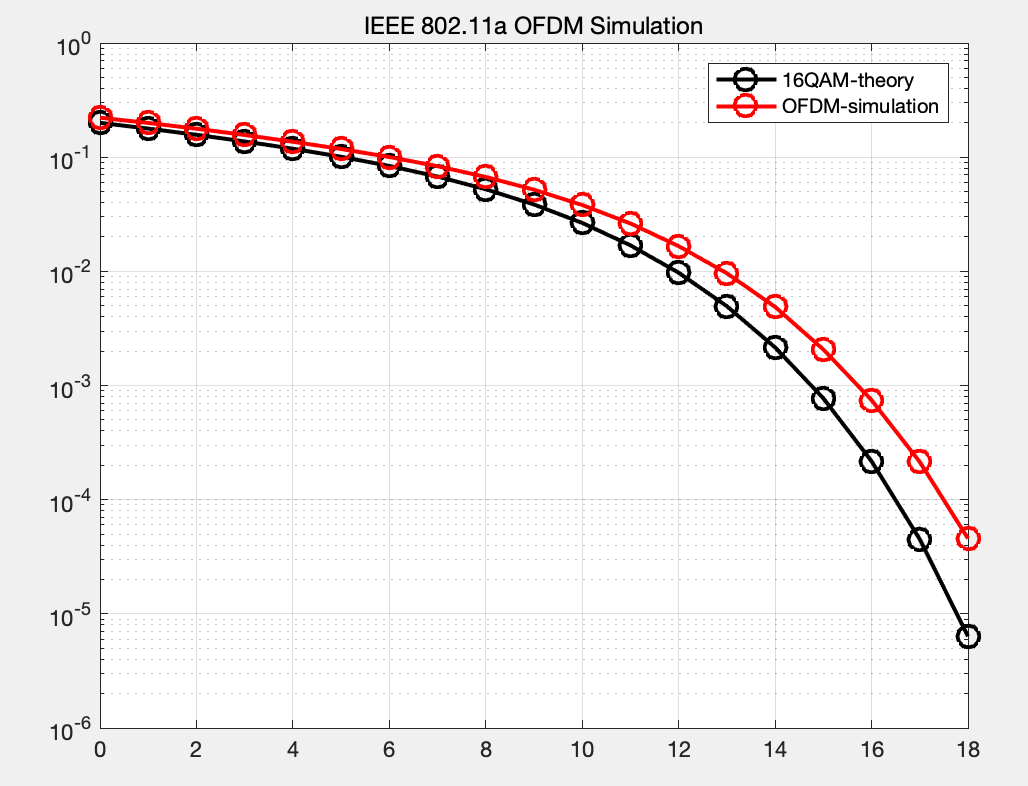
\includegraphics[width=0.7\linewidth]{64}
		\caption{64-QAM}
		\label{fig:64}
	\end{figure}
	
	The 64-QAM result is shown as Fig.6. 
\end{itemize}








\section{Conclusion}
\begin{itemize}
	\item We could clear see that \textbf{BPSK} and \textbf{QPSK} has exactly same curve no matter in geometry or data
	\item When $ \cfrac{E_0}{B_0} $ increases, EPR decreases. 
	\item As the \textcolor{blue}{order} of modulation increases,, the higher $ \cfrac{E_0}{B_0} $ is needed to reach the same EPR
	\item OFDM simulation result is not exact the same as theorically. Generally, OFDM result is a little higher than we thought. We call is as shift.
	\item The more \textcolor{blue}{order} is, those shift is less, which means we can match it well.
\end{itemize}
\subsection{Rethinking\& Answer to Questions in Lecture}

\begin{itemize}
	\item 
	\textcolor{blue}{\textbf{{Functions of OFDM Mapping}}}
	
	The \lstinline|ofdmmap.m| is as belows:
	\begin{lstlisting}
		function  data_out = ofdmmap(data_in, OFDM)
		
		%****************** variables *************************
		% data_in    : Input ch data
		% data_out : Output ch data
		% fftlen    : Length of FFT (points)
		% nd        : Number of OFDM symbols
		% *****************************************************
		% fftlen = 64;
		% nd = 6;
		
		data_out = zeros(OFDM.fftlen, OFDM.Nd);
		data_out(OFDM.ToneMap, :) = data_in(OFDM.subcarrier_order, :);
		
		end
	\end{lstlisting}
	As we can see, \lstinline|ofdmmap.m|  lets 48 channels of data map to IFFT input. The sender converts the transmitted digital signal into a mapping of subcarrier amplitude and phase. This ensures that adjacent coded bits are mapped to non-adjacent subcarriers and are mapped to important and non-important bits of the constellation respectively, avoiding long-term low-bit mapping.
	\item 
	\textcolor{blue}{\textbf{{Theoretical bit error rate curves of BPSK and QPSK are the same, why?}}}
	
	In textbook 4.8.4, we can find the explanation. Due to the formula about error rate:
	$$ \cfrac{E_b}{N_0}=\cfrac{S}{N}\cfrac{W}{R}$$
	QPSK can actually be represented by 2 orthogonal BPSK. Generally, QPSK can be divided into 2 sub streams which is $ I $ and $ Q $, $ I $ modulates $ cosw_0t $ and $ Q $ modulates $ sinw_0t $ at the half speed of origin. Attitude of $ I $ and $ Q $ is $ \cfrac{1}{\sqrt{2}} $ of $ A $. So each power of BPSK orthogonally is half of QPSK. Assume that bit speed of QPSK is $ R $ b/s, average power is $ S $ W, then each sub BPSK has bit speed of QPSK is $ R/2 $ b/s, average power is $ S/2 $ W. So
	$$  \cfrac{E_b}{N_0}=\cfrac{S/2}{N_0}\cfrac{W}{R/2}=\cfrac{S}{N}\cfrac{W}{R}$$
	Exactly same with former one. That's why QPSK and BPSK has the same error curve. The figure theorically is shown as Fig.7
	\begin{figure}[!h]
		\centering
		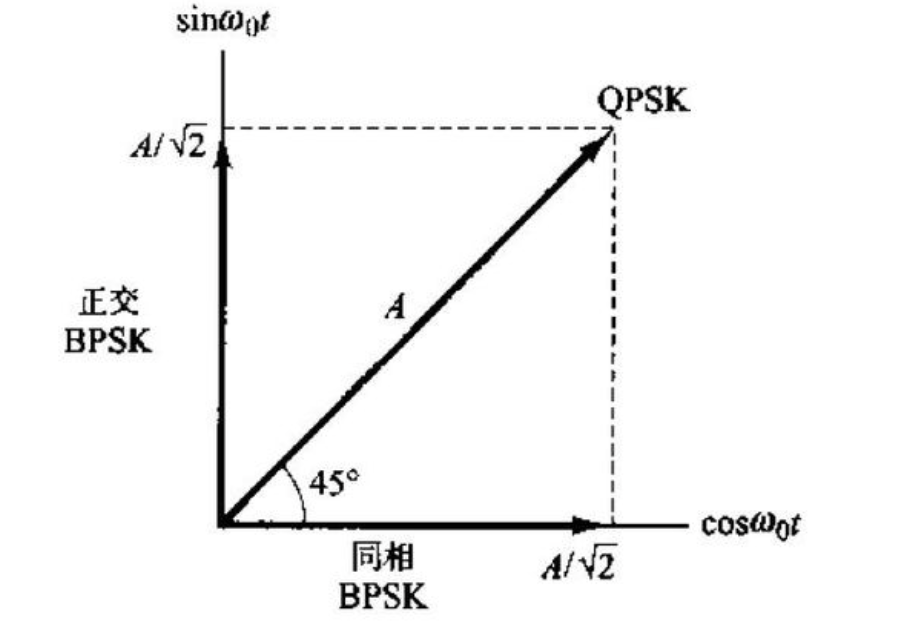
\includegraphics[width=0.7\linewidth]{10}
		\caption{QPSK and orthogonal BPSK }
		\label{fig:10}
	\end{figure}

	The result in MATLAB by bertools verifies as Fig.8:
	\begin{figure}[!h]
		\centering
		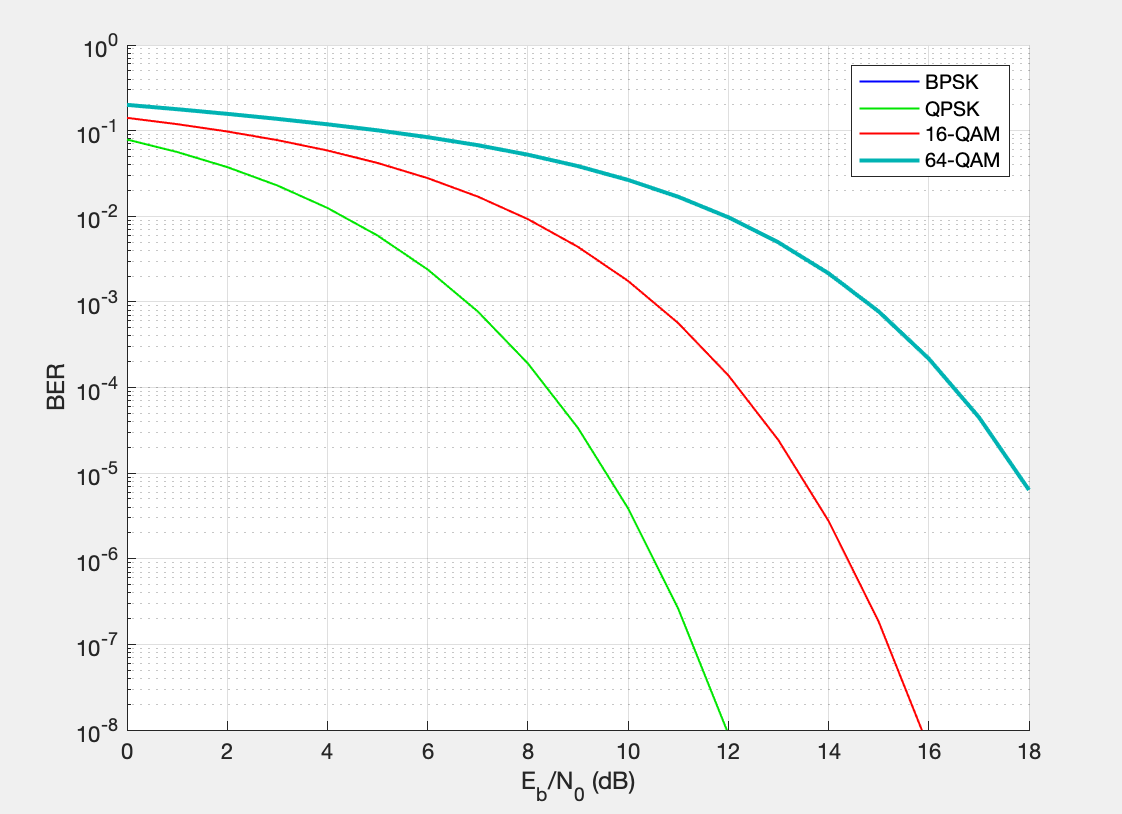
\includegraphics[width=0.7\linewidth]{9}
		\caption{Result theorically}
		\label{fig:9}
	\end{figure}

	\item 
	\textcolor{blue}{\textbf{{Try to explain the deviation between OFDM simulation error rate curve and theoretical curve}.}}
	
	The main reason of this is because the protect interval is introduced in OFDM, it is a kind of\textbf{ redundant information}, so compared with the theoretical error rate curve has happened. In this system, the protect interval uses Cyclic Prelix (CP). The latter part of the OFDM symbol is copied and added to the front of the OFDM symbol.
	
\end{itemize}



\subsection{Problems}

\begin{itemize}
\item  The source code provided is slow. So I rewrite another verisio nto speed it up. I seperates every occasion so it can work efficiently. Besides, using \textbf{tensorl normalization} and \textbf{vectorization} could help to increase parallelisim so improve process efficiency.
\item  Some functions in MATLAB is not so famillar with. I browsed official ducument and look deep in them. *REPORT: MATLAB 2016Rb has some bugs when using \lstinline|bertool|

\end{itemize}


\subsection{Achievements}
In this Lab, I have a clearer basic understanding of the communication system. We have a certain understanding of modulation and demodulation, and OFDM orthogonal frequency division multiplexing. The cost of the increase in frequency band utilization is the reduction of the signal-to-noise ratio. I have a certain understanding of the choice of various parameters of the system and how to compromise. At the same time, I know more about Matlab. The harvest is great.

Thanks for TAs for discussing and resolvutions!



%----------------------------------------------------------------------------------------


\end{document}